\subsection{AI và thị giác máy tính (Computer Vision)}

Trong một khung hình camera hành trình, người đi đường và người được phép xuất hiện rõ đều được phát hiện với cùng một nhãn là khuôn mặt. Nhãn này chỉ cho biết vị trí cần xử lý. Muốn biết nên giữ rõ khuôn mặt nào, hệ thống phải so với ảnh tham chiếu do người dùng cung cấp. Biển số cũng vậy: phải biết biển nằm ở đâu, rồi đọc xem chuỗi ký tự có thuộc danh sách miễn che hay không. Với video, quyết định che còn phải giữ được qua những khung hình mà đối tượng bị nhoè hoặc khuất một phần. Mục này trình bày các kiến thức nền cho ba việc đó.

\subsubsection{Phát hiện đối tượng và họ mô hình YOLO}

Mô hình phát hiện đối tượng nhận một ảnh và trả về danh sách dự đoán. Mỗi dự đoán gồm một hộp giới hạn $B=(x_1,y_1,x_2,y_2)$, nhãn lớp và điểm tin cậy. RedactFunnel chỉ quan tâm hai lớp: khuôn mặt và biển số. Hộp giới hạn vừa cho biết vùng cần che, vừa là phần ảnh được cắt ra để nhận dạng khi người dùng bật danh sách miễn che. Vì thế một hộp bị lệch có thể gây hai lỗi liên tiếp: để lộ một phần đối tượng, và cắt mất mắt hoặc ký tự cần cho bước nhận dạng.

YOLO là họ mô hình phát hiện một giai đoạn. Trong một lượt truyền qua mạng, phần \textit{backbone} trích đặc trưng ở nhiều độ phân giải, phần \textit{neck} kết hợp chi tiết không gian với ngữ cảnh, và phần \textit{head} dự đoán vị trí cùng lớp của đối tượng (Hình~\ref{fig:2-1}). YOLOv8 dùng đầu dự đoán tách nhánh và không cần hộp neo định trước. YOLO11 bổ sung các khối C3k2 và C2PSA vào backbone. YOLO26 đơn giản hoá nhánh hồi quy hộp và có thể xuất dự đoán trực tiếp, không cần bước loại hộp chồng lấn NMS riêng. Hậu tố \textit{n} (nano) và \textit{s} (small) chỉ cỡ mạng trong cùng một thế hệ.

\begin{figure}[!htbp]
\centering
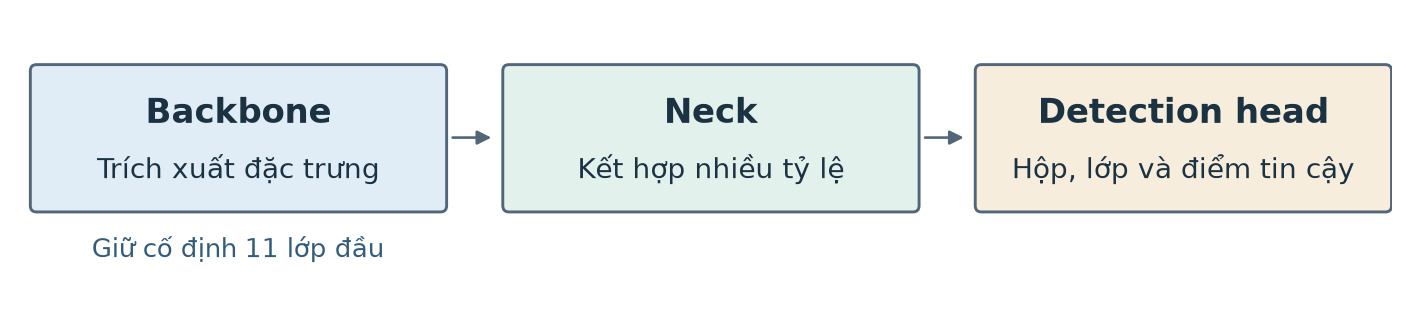
\includegraphics[width=0.92\textwidth]{figures/hinh-2-1-yolo.png}
\caption[Kiến trúc tổng quát của mô hình YOLO]{Kiến trúc tổng quát của mô hình YOLO. Khi tinh chỉnh YOLO26s với dữ liệu biển số, nhóm giữ cố định 11 lớp đầu thuộc backbone và chỉ cập nhật các lớp phía sau}
\label{fig:2-1}
\end{figure}

Với mặt người ở xa, kích thước ảnh đưa vào mạng quyết định còn lại bao nhiêu chi tiết sau khi thu nhỏ. Nhóm thử cùng một bộ trọng số YOLO11n ở hai kích thước, chọn ngưỡng sao cho precision mặt gần bằng nhau (0,781 và 0,780). Khi tăng từ 640 lên 1280 px, recall mặt tăng từ 0,477 lên 0,688, tức 21,1 điểm phần trăm.

\textbf{Ứng dụng trong dự án.} RedactFunnel dùng hai mô hình YOLO26n và YOLO26s tinh chỉnh ở 1280 px, ứng với hai chế độ phát hiện. Quá trình chọn mô hình được trình bày ở mục 4.3.

\subsubsection{Các chỉ số đánh giá mô hình phát hiện}

Gọi $G$ là hộp nhãn do người gán và $B$ là hộp dự đoán. Độ giao trên hợp (\textit{Intersection over Union}, IoU) đo mức trùng khớp của hai hộp:
\[
\operatorname{IoU}(B,G)=\frac{|B\cap G|}{|B\cup G|}.
\]

Với mỗi lớp, các dự đoán được xếp theo điểm tin cậy giảm dần, mỗi hộp nhãn được ghép với nhiều nhất một dự đoán. Cặp ghép có $\operatorname{IoU}\ge 0{,}5$ được tính là đúng ($TP$), dự đoán thừa là $FP$, đối tượng bị bỏ sót là $FN$. Precision cho biết trong các phát hiện được giữ lại có bao nhiêu phần đúng, recall cho biết trong các đối tượng cần tìm đã tìm được bao nhiêu, còn $F_1$ là trung bình điều hoà của hai đại lượng này:
\[
P=\frac{TP}{TP+FP},\qquad R=\frac{TP}{TP+FN},\qquad F_1=\frac{2PR}{P+R}.
\]

Thay đổi ngưỡng điểm tin cậy sẽ tạo ra đường precision--recall. $\mathrm{AP}_{50}$ là diện tích dưới đường này của một lớp khi ngưỡng IoU bằng 0,5, và $\mathrm{mAP}_{50}$ là trung bình $\mathrm{AP}_{50}$ của hai lớp. AP gộp nhiều ngưỡng, trong khi ảnh thật chỉ được xử lý ở một ngưỡng. Vì vậy khi so hai mô hình, nhóm chọn ngưỡng để precision mặt gần bằng nhau rồi so recall. Cách này cho biết mô hình nào tìm được nhiều mặt hơn với cùng mức báo nhầm.

Với bài toán ẩn danh, điều cần biết hơn cả là bao nhiêu diện tích của đối tượng đã được che. Trên một ảnh, gọi $M$ là hợp của các hộp che cùng lớp sau khi nới biên. Độ che phủ của hộp nhãn $G$ là $C(G)=|G\cap M|/|G|$. Với $N$ hộp nhãn, tỷ lệ đối tượng đạt tiêu chí che được định nghĩa là
\[
R_{\mathrm{privacy}}=\frac{1}{N}\sum_{i=1}^{N}\mathbf{1}\!\left[C(G_i)\ge 0{,}70\right].
\]

\begin{figure}[!htbp]
\centering
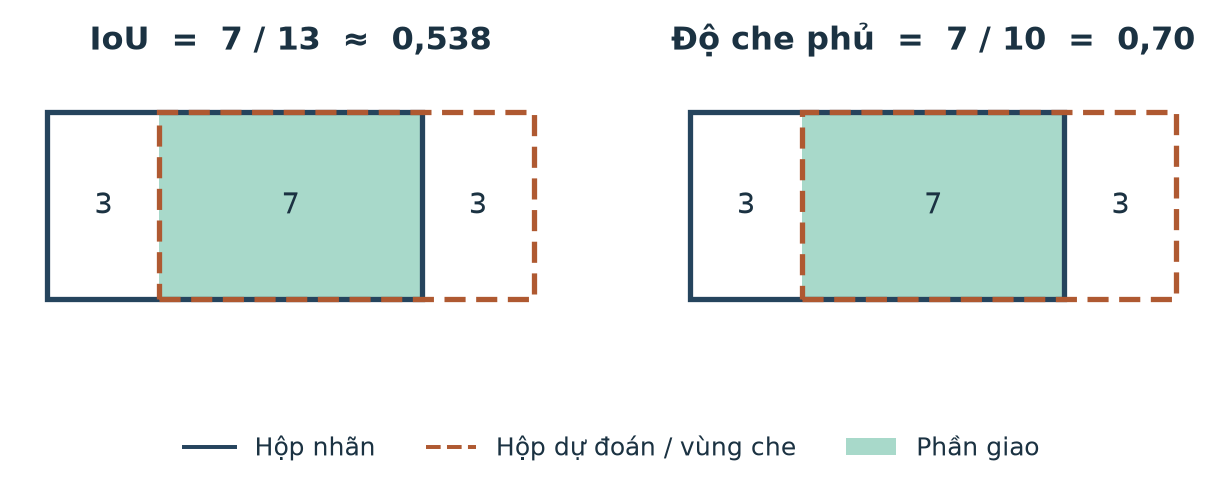
\includegraphics[width=0.85\textwidth]{figures/hinh-2-2-iou-che-phu.png}
\caption[IoU và độ che phủ]{IoU và độ che phủ của cùng một cặp hộp. Hai hộp rộng 10 đơn vị, lệch nhau 3 đơn vị: IoU bằng $7/13$, còn độ che phủ bằng $7/10$, vừa đạt ngưỡng 70\%}
\label{fig:2-2}
\end{figure}

Hai loại lỗi có hậu quả rất khác nhau. Một khuôn mặt bị bỏ sót sẽ xuất hiện nguyên vẹn trong ảnh công bố, còn một vùng nền bị che nhầm chỉ làm mất chi tiết. Vì vậy nhóm ưu tiên giảm bỏ sót, đồng thời theo dõi precision để việc che nhầm không quá nhiều. Ngưỡng 70\% là quy ước của đề tài. Việc có nhận ra người hay đọc được biển hay không còn phụ thuộc phần nào còn nhìn thấy và độ mạnh của phép che.

\textbf{Ứng dụng trong dự án.} Mọi mô hình và công cụ ở Chương 4 đều được so trên cùng tập ảnh, ở cùng mức precision, theo tỷ lệ đối tượng đạt tiêu chí che.

\subsubsection{Nhận diện khuôn mặt bằng vector đặc trưng (face embedding)}

Để biết một khuôn mặt có thuộc danh sách miễn che hay không, mạng nhận diện ánh xạ khuôn mặt thành một vector đặc trưng. ArcFace (Deng và cộng sự, 2019) là phương pháp huấn luyện thêm một biên góc vào hàm mất mát, giúp các danh tính tách xa nhau hơn trong không gian đặc trưng. RedactFunnel dùng mạng MobileFaceNet có sẵn trọng số, chạy bằng ONNX Runtime, sinh vector 512 chiều đã chuẩn hoá $L_2$.

Góc nghiêng của đầu và vị trí mắt thường khác nhau giữa ảnh tham chiếu và ảnh cần che. Trước khi tính vector, YuNet tìm năm điểm mốc gồm hai mắt, đầu mũi và hai khoé miệng. Từ đó hệ thống xoay và co giãn khuôn mặt về vị trí chuẩn trên ảnh $112\times112$ px. Nếu không tìm đủ điểm mốc, vùng mặt được đổi kích thước trực tiếp. Tác động của bước căn chỉnh được đánh giá ở mục 4.7.

Với vector $\mathbf{u}$ của khuôn mặt đang xét và vector tham chiếu $\mathbf{v}$, độ tương đồng cosine là
\[
s(\mathbf{u},\mathbf{v})=\frac{\mathbf{u}^{\mathsf T}\mathbf{v}}{\|\mathbf{u}\|_2\,\|\mathbf{v}\|_2}.
\]

Hệ thống lấy điểm cao nhất trong các ảnh tham chiếu và so với ngưỡng mặc định 0,45. Người lạ vượt ngưỡng sẽ bị giữ rõ nhầm, còn người trong danh sách không đạt ngưỡng sẽ bị che. Ở đây cần phân biệt hai ngưỡng: hạ ngưỡng phát hiện giúp tìm thêm mặt cần bảo vệ, nhưng hạ ngưỡng so khớp lại có thể để lọt người lạ. Vì thế hai ngưỡng được đánh giá riêng.

\textbf{Ứng dụng trong dự án.} ArcFace và YuNet chỉ được dùng khi người dùng tải lên ảnh mẫu. Nếu chỉ yêu cầu che toàn bộ khuôn mặt, hệ thống bỏ qua bước này.

\subsubsection{Nhận dạng ký tự quang học cho biển số Việt Nam}

Biển số dài của ô tô có một dòng, đọc từ trái sang phải. Biển vuông của xe máy và một số ô tô có hai dòng, nên bộ nhận dạng phải giữ đúng thứ tự dòng trên rồi mới đến dòng dưới (Hình~\ref{fig:2-3}). Ngoài bố cục, màu nền cũng khác nhau, ví dụ biển nền vàng của xe kinh doanh vận tải hay biển nền xanh của xe công vụ, khiến độ tương phản của chữ thay đổi.

\begin{figure}[!htbp]
\centering
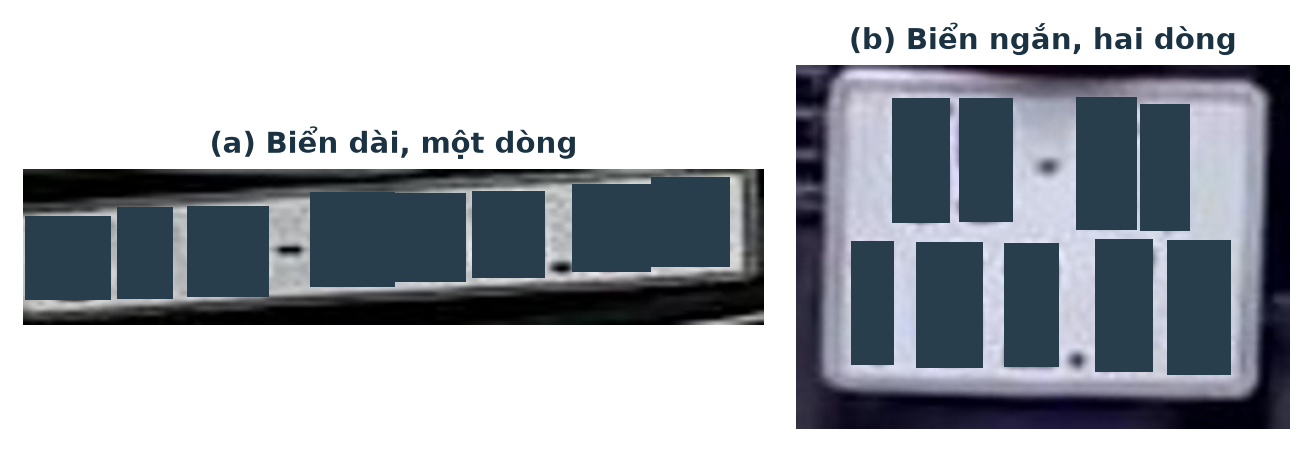
\includegraphics[width=0.8\textwidth]{figures/hinh-2-3-bien-so.png}
\caption[Các dạng biển số Việt Nam]{Hai dạng biển số Việt Nam: (a) biển dài một dòng, (b) biển vuông hai dòng. Ký tự được phủ ô đậm để không lộ số đăng ký}
\label{fig:2-3}
\end{figure}

Do YOLO đã xác định vị trí biển, hệ thống chỉ dùng phần nhận dạng của PP-OCRv4 thông qua RapidOCR, bỏ qua bước phát hiện chữ. Bộ nhận dạng này đọc mỗi lần một dòng, nên mỗi biển được đọc theo hai cách: đọc nguyên vùng biển, và chia đôi theo chiều cao rồi đọc từng nửa. Ảnh đưa vào được kéo ngang 1,3 lần để các chữ số giống nhau đứng cạnh nhau không bị gộp. Cách đọc nào có điểm tin cậy cao hơn thì được chọn.

Sau khi đọc, chuỗi được chuyển thành chữ hoa và bỏ dấu phân cách. Biển chỉ được miễn che khi điểm OCR từ 0,50 trở lên và chuỗi khớp với danh sách. Vì một lần đọc sai vẫn có thể tạo ra chuỗi giống biển được phép, mục 4.6 đánh giá riêng độ chính xác khi đọc và tỷ lệ miễn che nhầm.

\textbf{Ứng dụng trong dự án.} RapidOCR chạy trên ONNX Runtime, dùng chung môi trường với ArcFace nên không phải thêm một thư viện suy luận khác.

\subsubsection{Theo dõi đối tượng và xử lý video}

Trong video hành trình, một biển số có thể rõ ở khung này nhưng nhoè ở khung kế tiếp. Nếu xử lý từng khung riêng lẻ, vết che có thể biến mất đúng lúc điểm phát hiện giảm. ByteTrack (Zhang và cộng sự, 2022) giải quyết việc này bằng cách nối các hộp qua thời gian thành quỹ đạo. Bộ lọc Kalman dự báo vị trí ở khung kế tiếp, các quỹ đạo được ghép với phát hiện điểm cao trước, rồi mới dùng phát hiện điểm thấp để nối những quỹ đạo còn lại. Một mã quỹ đạo cho biết đối tượng liên tục trong đoạn video, nhưng việc đối tượng có được miễn che hay không vẫn phải dựa vào khuôn mặt hoặc biển số.

RedactFunnel xử lý video hai lượt. Lượt đầu phát hiện, nối quỹ đạo và lưu lại các vùng ảnh tốt nhất để xét miễn che. Lượt sau dựng vết che trên từng khung và nội suy ở những khoảng mất dấu ngắn. Phát hiện chưa được ByteTrack gán mã vẫn được che, nên một người chỉ xuất hiện thoáng qua cũng không bị bỏ sót.

Về tệp video, công cụ ffprobe đọc độ phân giải, tốc độ khung hình và luồng âm thanh, OpenCV giải mã từng khung, còn FFmpeg mã hoá kết quả theo chuẩn H.264. Âm thanh gốc được ghép lại nguyên vẹn, không mã hoá lại, và siêu dữ liệu của tệp nguồn được xoá. Thời gian xử lý tăng theo thời lượng video, trong khi một job ảnh chỉ có một ảnh.

\textbf{Ứng dụng trong dự án.} Sự khác biệt này là lý do nhóm tách hàng đợi ảnh và video thành hai nhóm worker, co giãn độc lập với nhau như trình bày ở Chương 3.
